\documentclass[mathserif,serif]{beamer}
\usepackage[ngerman]{babel}
%\usepackage[scale=0.75]{geometry}
\usepackage{graphics}
\usepackage{graphicx}
\usepackage{amsmath}
\usepackage{amssymb}
\usepackage{subfigure} 
\usepackage[utf8]{inputenc}
\usepackage{amsmath}
\usepackage{amsfonts}
\usepackage{amssymb}
\usepackage{fancyhdr}
\usepackage[hang, center, nooneline]{caption}
\usepackage{epstopdf}
\usepackage{color}
\usepackage{subfigure}
\usepackage{wrapfig}
\usepackage{color}															 
\usepackage{colortbl}
\usepackage{siunitx}
\usepackage{fancybox}
\usepackage{relsize}
\usepackage{booktabs}
\usepackage{tikz}
\usepackage{textpos}
\usepackage{colortbl}

\definecolor{TUeRed}{RGB}{170,0,0}
\definecolor{TUeBlue}{RGB}{0,68,170}

\addtobeamertemplate{frametitle}{}{% 
\begin{textblock*}{100mm}(.95\textwidth,-1cm) \tikz {\fill[white] (0,0) -- %
(2cm,0) -- (2cm,1.1cm) -- (0.5cm,1.1cm) -- cycle;\node[TUeBlue] at %
(0.8cm,0.5cm) {\normalsize\insertframenumber};} \end{textblock*} }

\setbeamercolor{frametitle}{bg=TUeBlue}
\setbeamercolor{frametitle}{fg=white}

  
%EIGENE FOOTLINE (OHNE GESAMTSEITENZAHL) 
%\setbeamertemplate{footline} 
%{ 
%\leavevmode% 
%\hbox{% 
%\begin{beamercolorbox}[wd=.333333\paperwidth,ht=2.25ex,dp=1ex,center]{author in head/foot}% 
%\usebeamerfont{author in head/foot}\insertshortauthor~~ 
%\end{beamercolorbox}% 
%\begin{beamercolorbox}[wd=.333333\paperwidth,ht=2.25ex,dp=1ex,center]{title in head/foot}% 
%\usebeamerfont{title in head/foot}\insertshorttitle 
%\end{beamercolorbox}% 
%\begin{beamercolorbox}[wd=.333333\paperwidth,ht=2.25ex,dp=1ex,right]{date in head/foot}% 
%\usebeamerfont{date in head/foot}\insertshortdate{}
%\end{beamercolorbox}}% 
%\vskip0pt% 
%}

\setbeamertemplate{footline}[text line]{%
  \parbox{\linewidth}{\vspace*{-8pt}\hspace*{-5mm}\insertshortauthor\hfill Particles in a Potential\hfill\insertdate}}

\beamertemplatenavigationsymbolsempty

\author{Christopher Deutsch and Philip Hauer}
\title{Particles in a Potential}
\date{30. March 2016}
\subtitle{{\small Computational Physics}}

\begin{document}
\frame[plain]{\titlepage}
\setcounter{framenumber}{0}
\begin{frame}
	\frametitle{Introduction - Particles in a Potential}
		\begin{columns}
		\column[c]{.50\textwidth}
			\centering
			Core of this project:
			\begin{itemize}
				\item positive and negative particles
				\item interaction via potential
				\item analysis with a Random-Walk Metropolis algorithm
				\item study of temperature dependence
				\item further thoughts (e.g. other potentials)
			\end{itemize}
		\column[c]{.50\textwidth}
			
	\end{columns}
\end{frame}


% % % % % % % % % % % % Philip Intro

%Hier Folien


% % % % % % % % % % % % Chris Background & Implementation

%Hier Folien
\begin{frame}{Canonical ensemble}
	\begin{columns}
		\column[c]{0.5\textwidth}
			\begin{itemize}
				\setlength\itemsep{1.5em}
				\item statistical ensemble
				\item systems with constant:
				\begin{itemize}
					\item number of particles~$N$
					\item volume~$V$
					\item temperature~$T$
				\end{itemize}
				
				\item probabilistic description
			\end{itemize}
		
			
		\column[c]{0.5\textwidth}
			\centering
			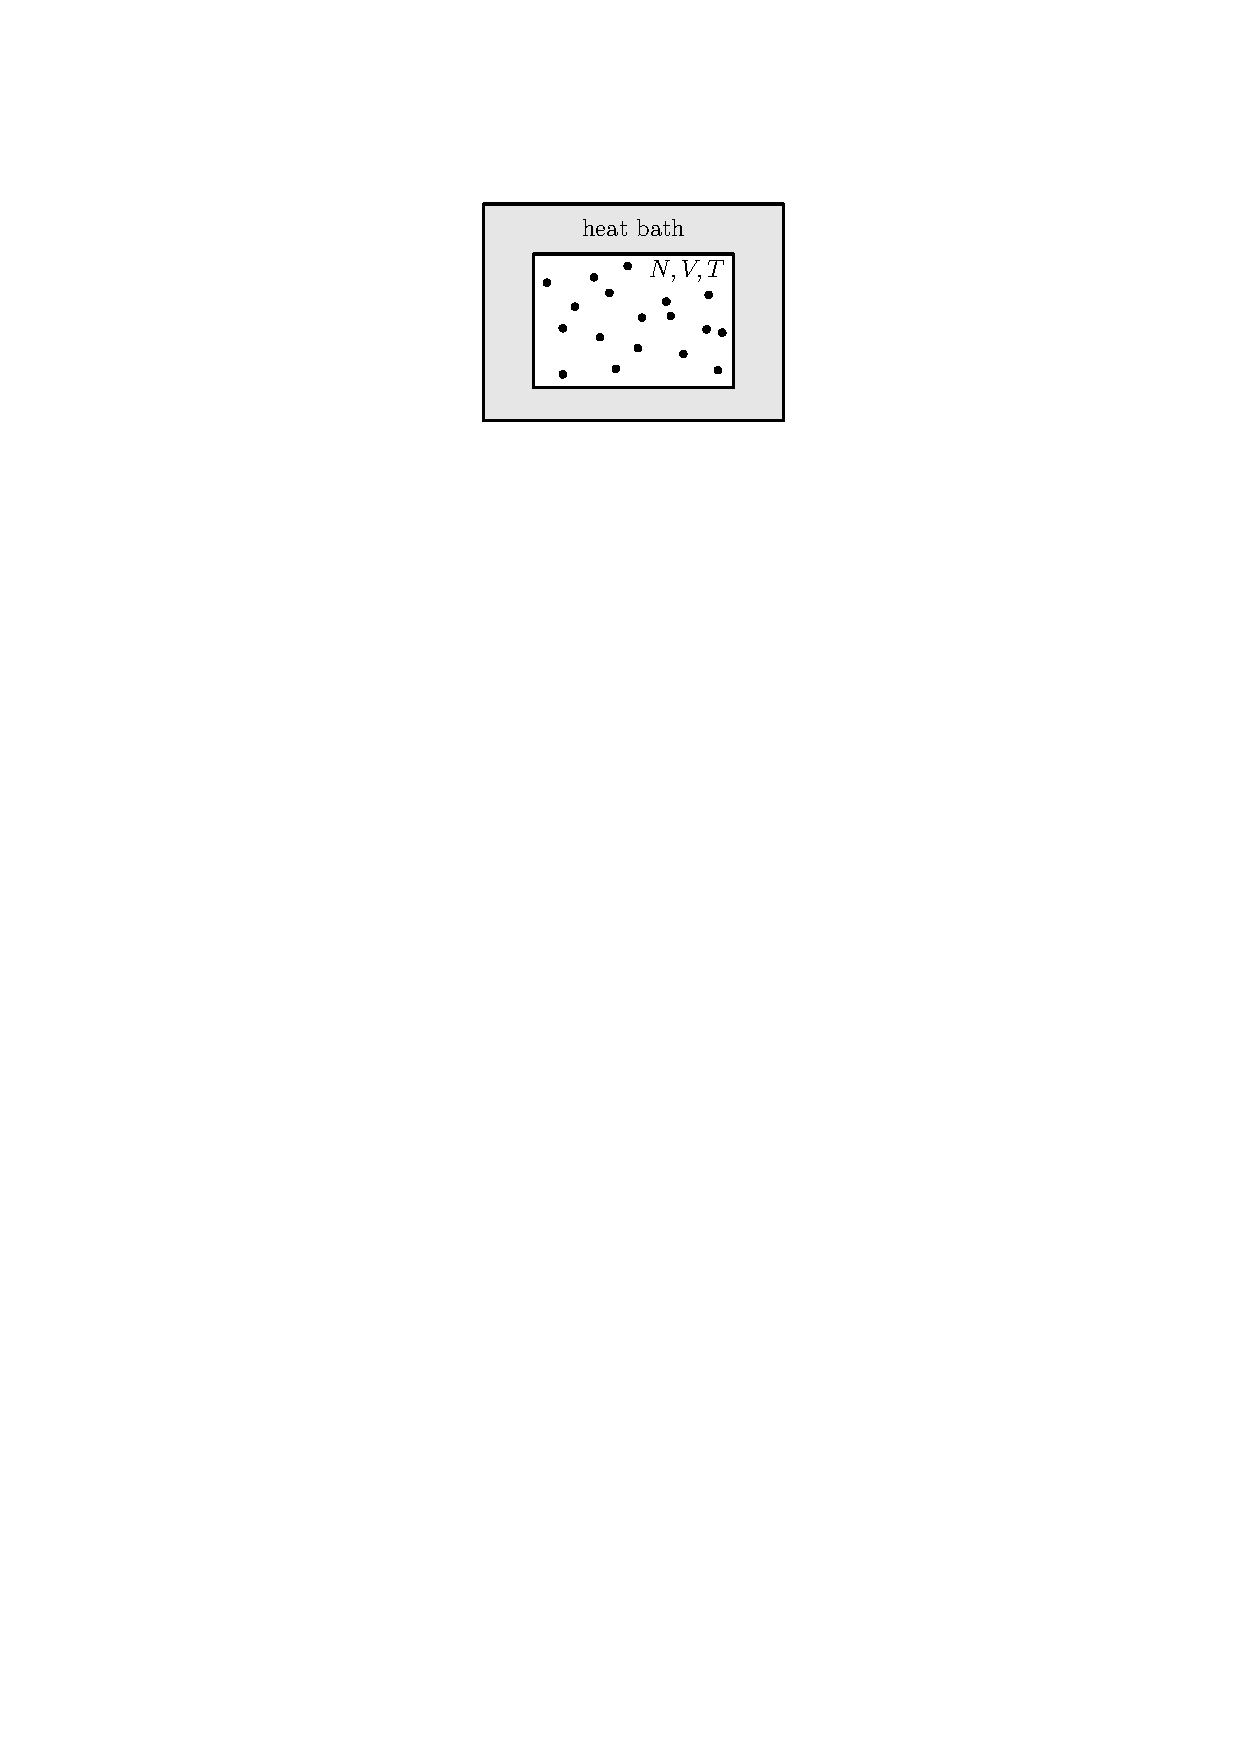
\includegraphics[width=0.9\textwidth]{./figures/canonical_ensemble.pdf}
		
	\end{columns}
\end{frame}

\begin{frame}{Canonical ensemble}
	\begin{itemize}
		\setlength\itemsep{2.0em}
		\item probability density:
		\begin{align*}
			P(E) = \frac{1}{Z} \exp\left[ - \beta E \right] \qquad \beta := \frac{1}{k_\mathrm{B} T}
		\end{align*}
		$E$: total energy of system\\
		$Z$: canonical partition function
		
		\item examine temperature dependence:
		\begin{itemize}
			\item sample states from distribution
			\item calculate expectation values of observables
		\end{itemize}
	\end{itemize}
\end{frame}

\begin{frame}{Metropolis algorithm}
	\begin{itemize}
		\setlength\itemsep{1.5em}
		\item MCMC method for sampling from (complicated) distributions
		\item correlated sequence of random samples
		\begin{itemize}
			\item used to approximate distribution
		\end{itemize}
		\item Random-Walk Metropolis
	\end{itemize}

\end{frame}

\begin{frame}{Random-Walk Metropolis algorithm}
	Given target density $P(x)$ and initial state $x_0$:
	\vspace*{0.2cm}
	\begin{enumerate}
		\setlength{\itemsep}{1.5em}
		\item Trial change:
		\begin{itemize}
			\item generate new state $y$ according to symmetric proposal distribution $q(Y|x_n)$
		\end{itemize}
		
		\item Accept-reject:
		\begin{itemize}
			\item accept with probability:
			\begin{align*}
				\alpha = \min\left\{ \frac{P(y)}{P(x_n)}, 1 \right\}
			\end{align*}
		\end{itemize}
		
		\item Repeat
	\end{enumerate}		
\end{frame}

\begin{frame}{Implementation}
	\begin{columns}
		\column[c]{0.5\textwidth}
			\begin{itemize}
				\item<1-> box with side length~$L$
				\item<2-> random initial state
				\item<3-> select particle at random and calculate contribution to potential energy~$V$
				\item<4-> propose new state in box with side length~$\Delta$
				\item<5-> accept with probability
				\begin{align*}
					\alpha = \exp\left[ -\beta (V_\mathrm{prop.} - V_\mathrm{cur.}) \right]
				\end{align*}
			\end{itemize}
		\column[c]{0.5\textwidth}
			\centering
			\includegraphics<1>{./figures/impl_01.pdf}
			\includegraphics<2>{./figures/impl_02.pdf}
			\includegraphics<3>{./figures/impl_03.pdf}
			\includegraphics<4>{./figures/impl_04.pdf}
			\includegraphics<5>{./figures/impl_05.pdf}
			\includegraphics<6>{./figures/impl_06.pdf}
	\end{columns}
\end{frame}


% % % % % % % % % % % % Philip Intro Tempdep & Potentials

%Hier Folien


% % % % % % % % % % % % Chris 4.2 Analysis & avg pair distance

%Hier Folien


% % % % % % % % % % % % Philip Coulomb 2D 3D & Visualizations

%Hier Folien


% % % % % % % % % % % % Chris LJ 2D 3D & Visualizations

%Hier Folien


% % % % % % % % % % % % Philip (+ Chris) Conclusion

%Hier Folien


\end{document}